% !TEX program = XeLaTeX
% !TEX encoding = UTF-8
% @brief: group meeting slide
% @author: Zihang Xu
% @reference: https://github.com/latexstudio/HUST-Beamer-Theme
% @date: 2024-12-02

\documentclass{beamer}
\usepackage[T1]{fontenc}
\usepackage{
    ctex,
    xeCJK,
    natbib,
    xcolor,
    amsmath,
    caption,
    booktabs,
    calligra,
    hyperref,
    graphicx,
    latexsym,
    listings,
    multicol,
    multirow,
    pstricks,
    stackengine
}
\usepackage{HUST}

\setCJKfamilyfont{hei}{SimHei}

\def\cmd#1{\texttt{\color{red}\footnotesize $\backslash$#1}}
\def\env#1{\texttt{\color{blue}\footnotesize #1}}
\definecolor{deepblue}{rgb}{0,0,0.5}
\definecolor{deepred}{rgb}{0.6,0,0}
\definecolor{deepgreen}{rgb}{0,0.5,0}
\definecolor{halfgray}{gray}{0.55}

\lstset{
    basicstyle=\ttfamily\small,
    keywordstyle=\bfseries\color{deepblue},
    emphstyle=\ttfamily\color{deepred},
    stringstyle=\color{deepgreen},
    numbers=left,
    numberstyle=\small\color{halfgray},
    rulesepcolor=\color{red!20!green!20!blue!20},
    frame=shadowbox,
}

\author{徐梓航}
\title{Benchmarking Large Language Models in Retrieval-Augmented Generation}
\subtitle{
    \scriptsize
    Jiawei Chen\scriptsize\texorpdfstring{$^{@ISCAS}$}{\textit{@ISCAS}}
    \normalfont
    , Hongyu Lin\scriptsize\texorpdfstring{$^{@ISCAS
    }$}{\textit{@ISCAS}}
    \normalfont
    , et al. AAAI, 2024
}
\institute{华中科技大学计算机科学与技术学院}
\date{2024年12月09日}

\begin{document}

\begin{frame}
    \titlepage
    \begin{figure}[htpb]
        % \begin{center}
        %     
\includegraphics[width=0.2\linewidth]{images/templates/HUST_LOGO.eps}
        % \end{center}
    \end{figure}
\end{frame}

\begin{frame}
    \tableofcontents[sectionstyle=show,subsectionstyle=show/shaded/hide,subsubsectionstyle=show/shaded/hide]
\end{frame}

\section{Introduction \& Challenge}

\begin{frame}
    \begin{figure}[h]
        \centering
        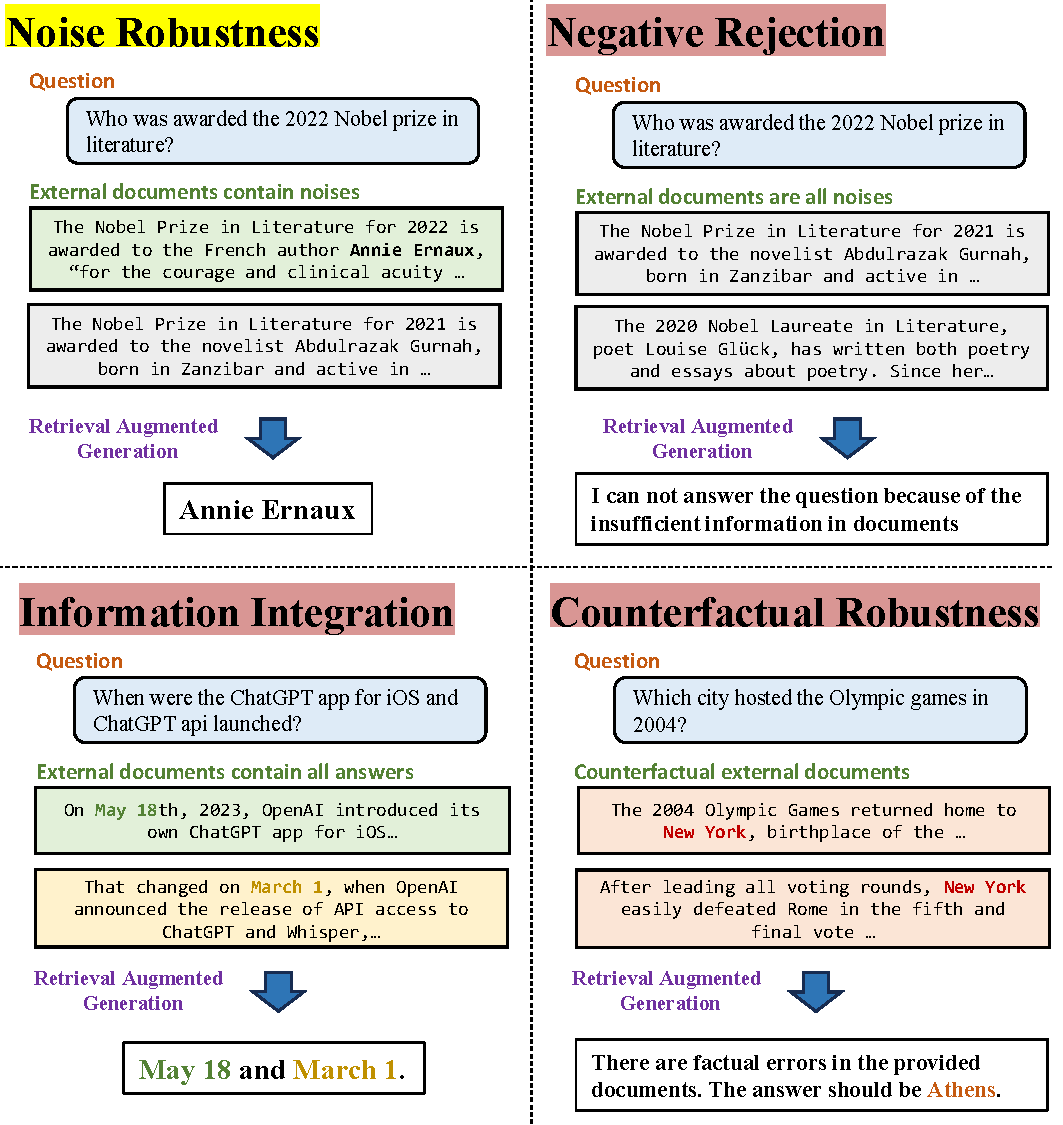
\includegraphics[height=.75\textheight]{./images/figures/intro.pdf}
        \captionsetup{font={tiny}}
        \caption{Four kinds of abilities required for ARG of LLMs.}
    \end{figure}
    \begin{itemize}
        \item {\colorbox{yellow}{噪声鲁棒性}(Noise Robustness):能否有效处理和忽略无用信息。}
    \end{itemize}
\end{frame}

\begin{frame}
    \begin{figure}[h]
        \centering
        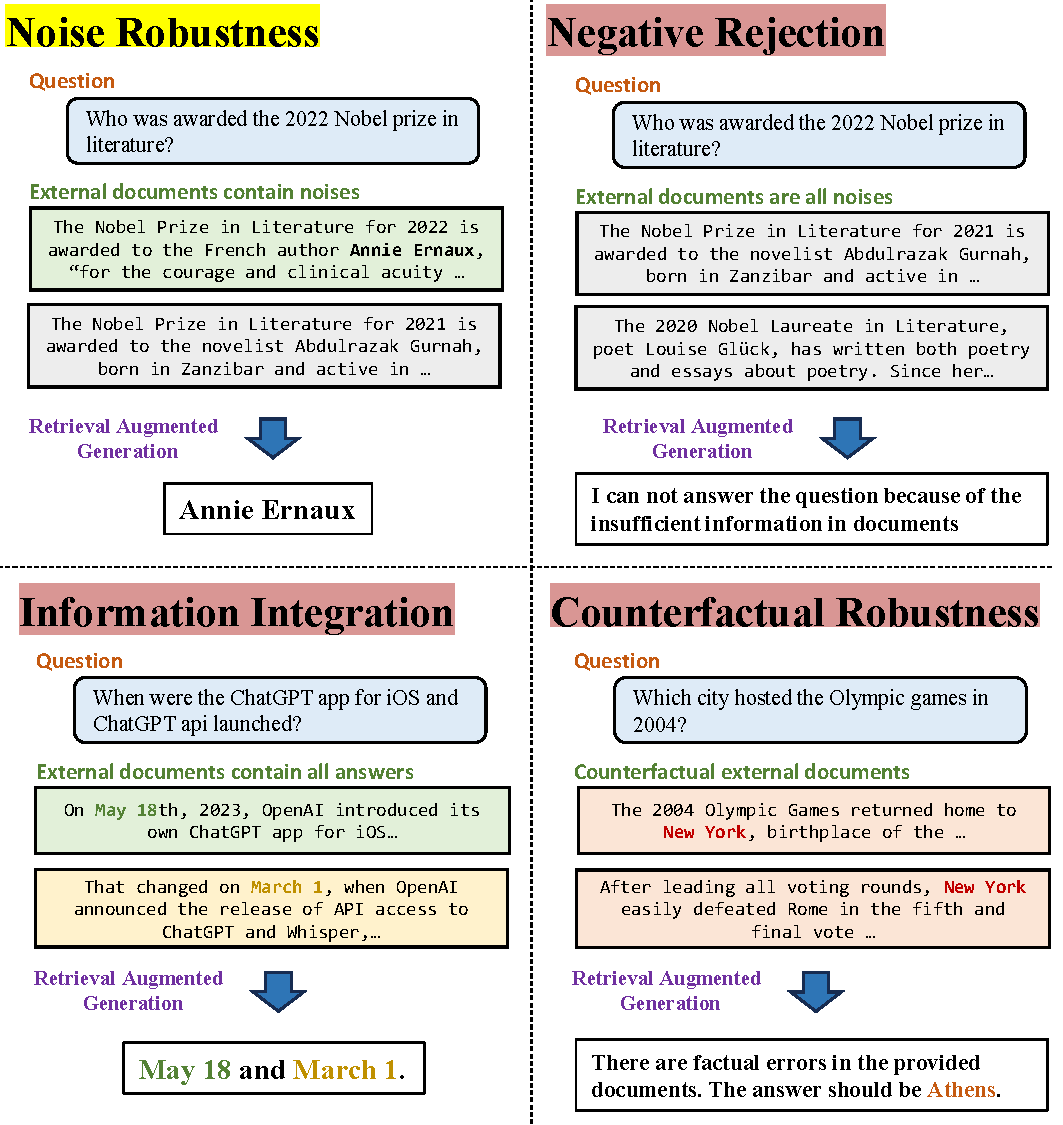
\includegraphics[height=.74\textheight]{./images/figures/intro.pdf}
        \captionsetup{font={tiny}}
        \caption{Four kinds of abilities required for ARG of LLMs.}
    \end{figure}
    \begin{itemize}
        \item {\colorbox{red}{负面拒绝}(Negative Rejection):确保在没有足够信息时不会生成不准确或虚假的答案。}
    \end{itemize}
\end{frame}

\begin{frame}
    \begin{figure}[h]
        \centering
        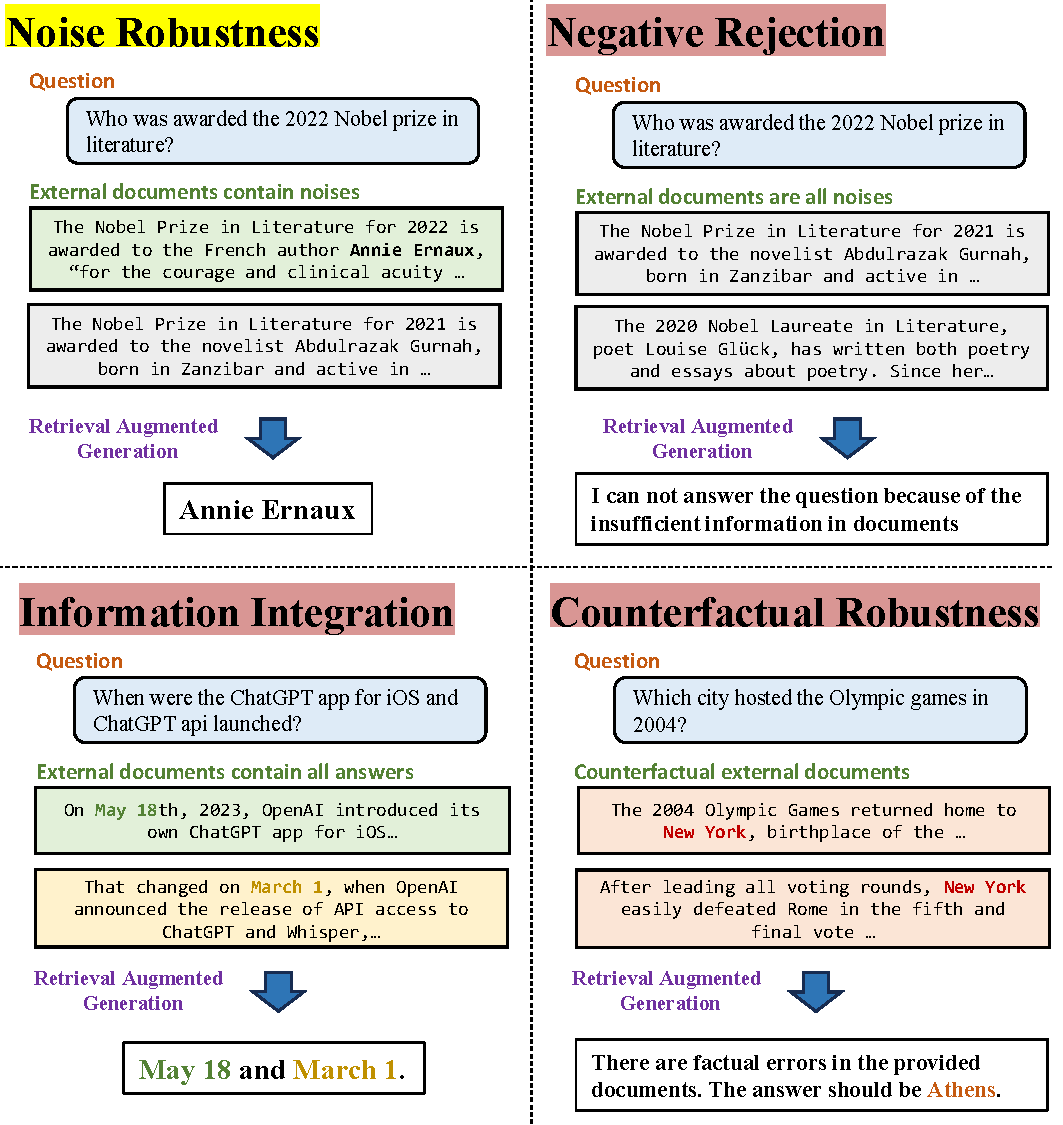
\includegraphics[height=.74\textheight]{./images/figures/intro.pdf}
        \captionsetup{font={tiny}}
        \caption{Four kinds of abilities required for ARG of LLMs.}
    \end{figure}
    \begin{itemize}
        \item {\colorbox{red}{信息整合}(Information Integration):测试处理多源信息的能力。}
    \end{itemize}
\end{frame}

\begin{frame}
    \begin{figure}[h]
        \centering
        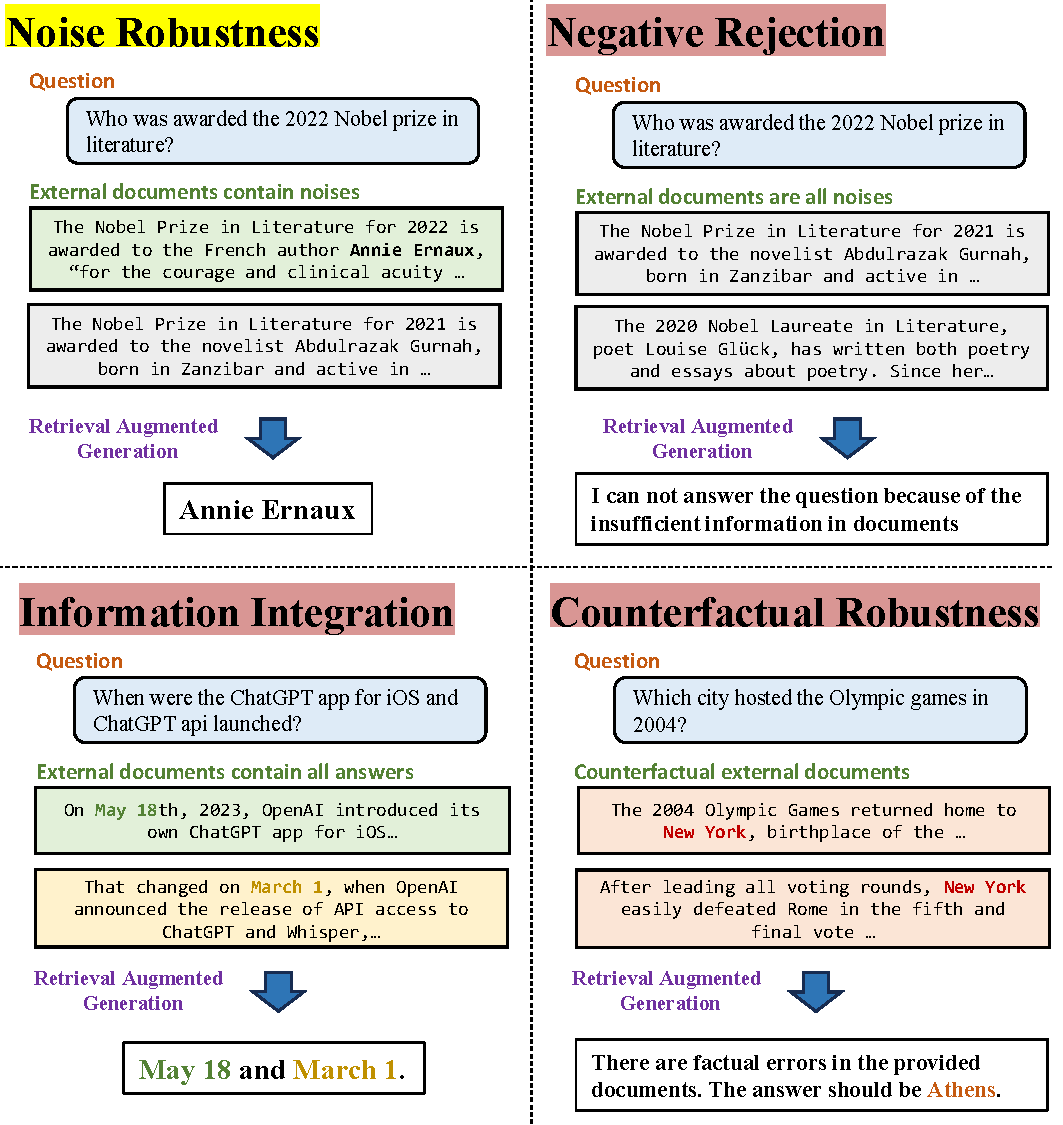
\includegraphics[height=.75\textheight]{./images/figures/intro.pdf}
        \captionsetup{font={tiny}}
        \caption{Four kinds of abilities required for ARG of LLMs.}
    \end{figure}
    \begin{itemize}
        \item {\colorbox{red}{反事实鲁棒性}(Counterfactual Robustness):在面对误导性信息时能够作出正确的判断。}
    \end{itemize}
\end{frame}

\section{Methods}

\begin{frame}
    \begin{figure}[h]
        \centering
        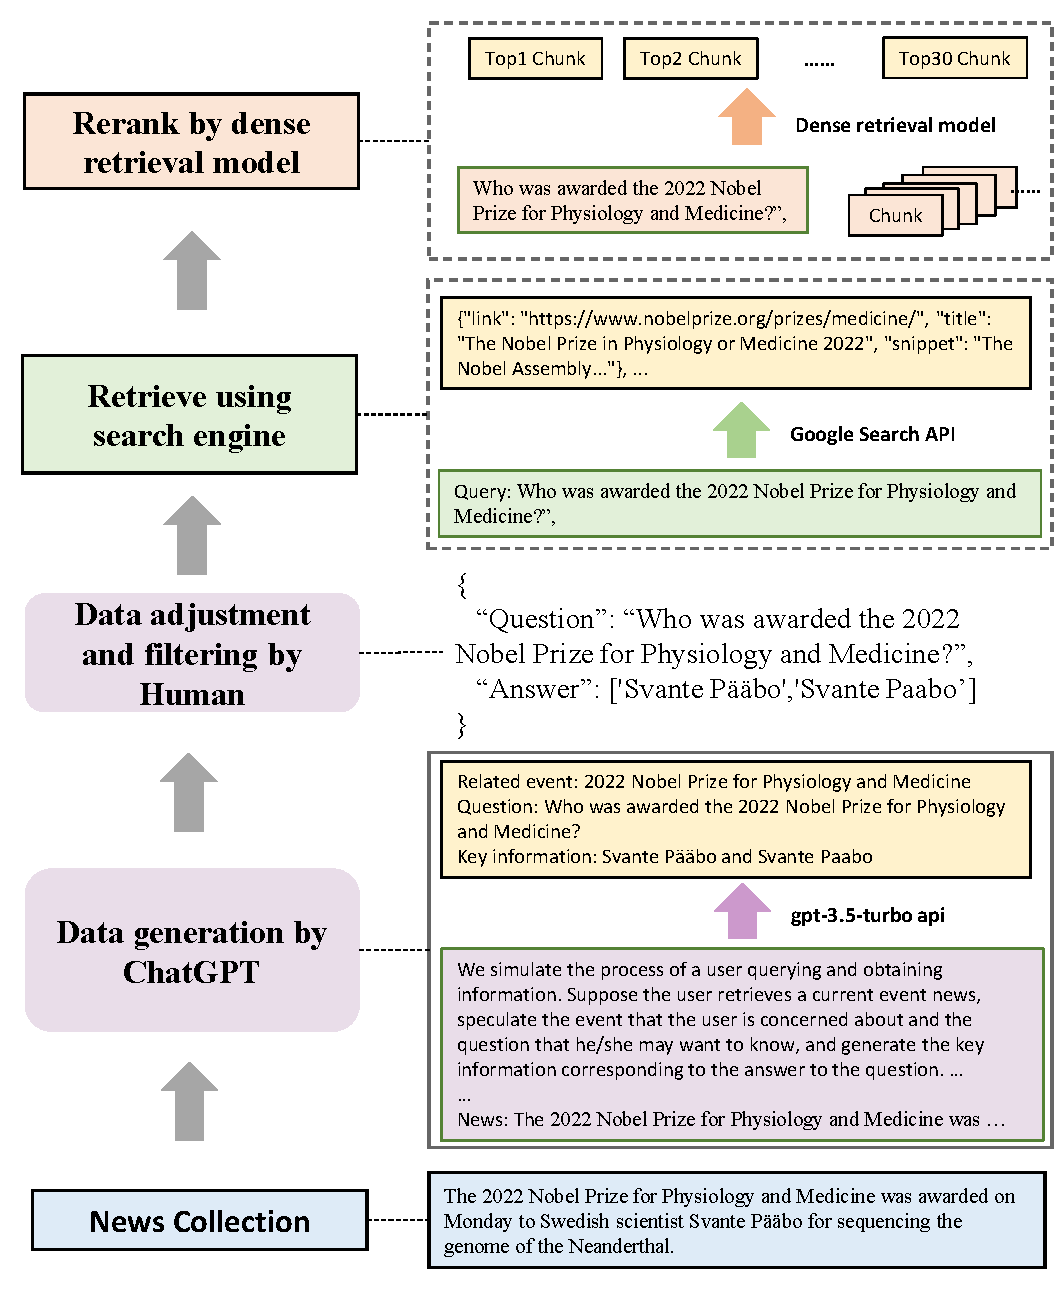
\includegraphics[height=.75\textheight]{./images/figures/data.pdf}
        \captionsetup{font={tiny}}
        \caption{The process of data generation.}
    \end{figure}
    \begin{itemize}
        \item {\bfseries{QA instances generation}}
    \end{itemize}
\end{frame}

\begin{frame}
    \begin{figure}[h]
        \centering
        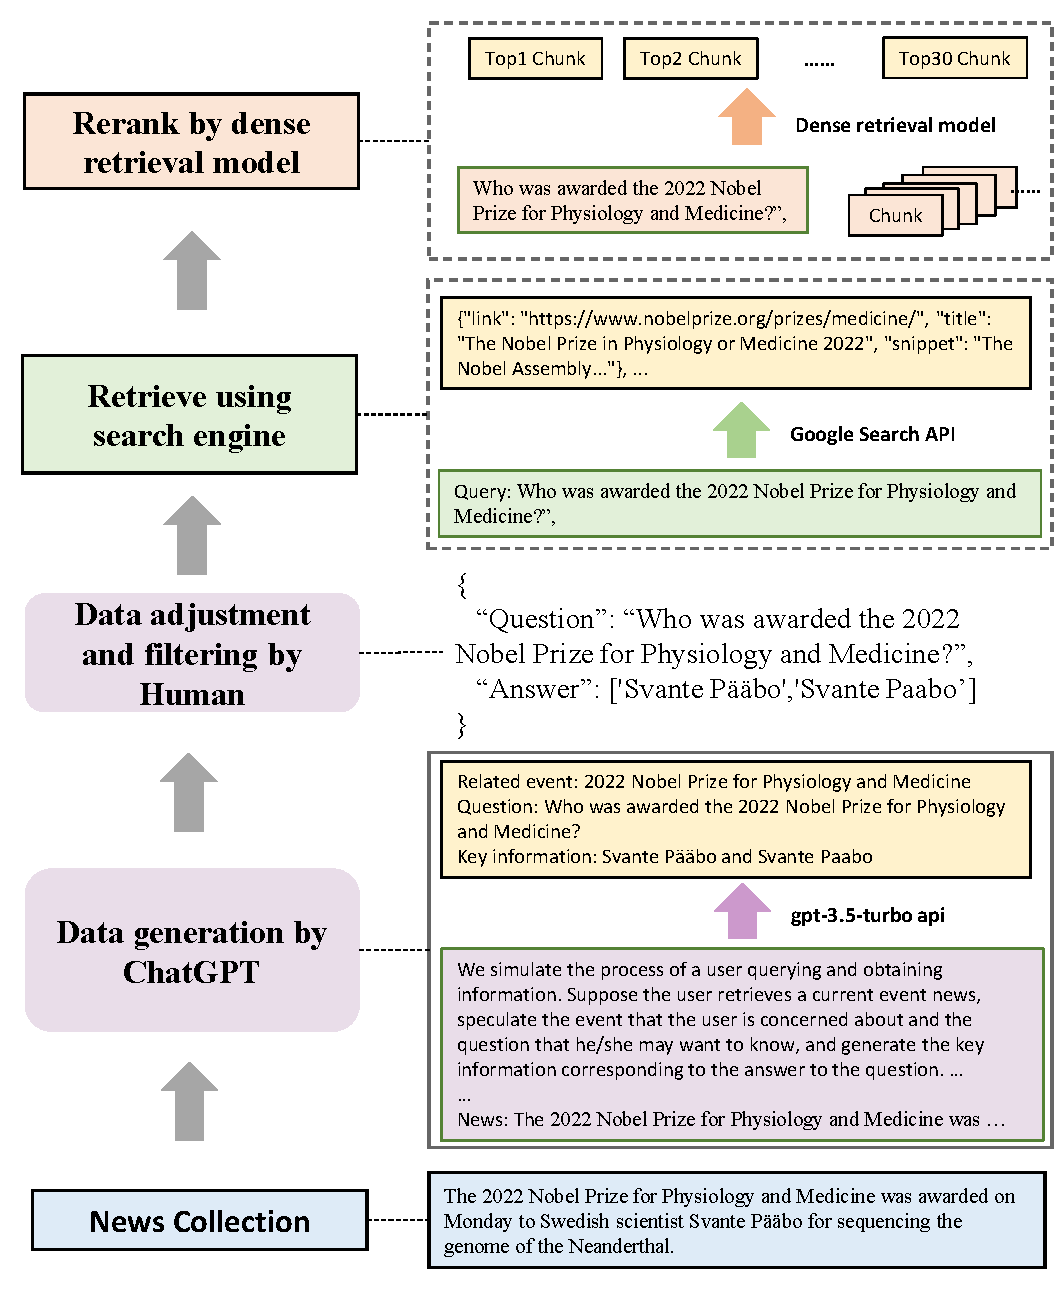
\includegraphics[height=.75\textheight]{./images/figures/data.pdf}
        \captionsetup{font={tiny}}
        \caption{The process of data generation.}
    \end{figure}
    \begin{itemize}
        \item {\bfseries{Retrieve using search engine}}
    \end{itemize}
\end{frame}

\begin{frame}
    \begin{figure}[h]
        \centering
        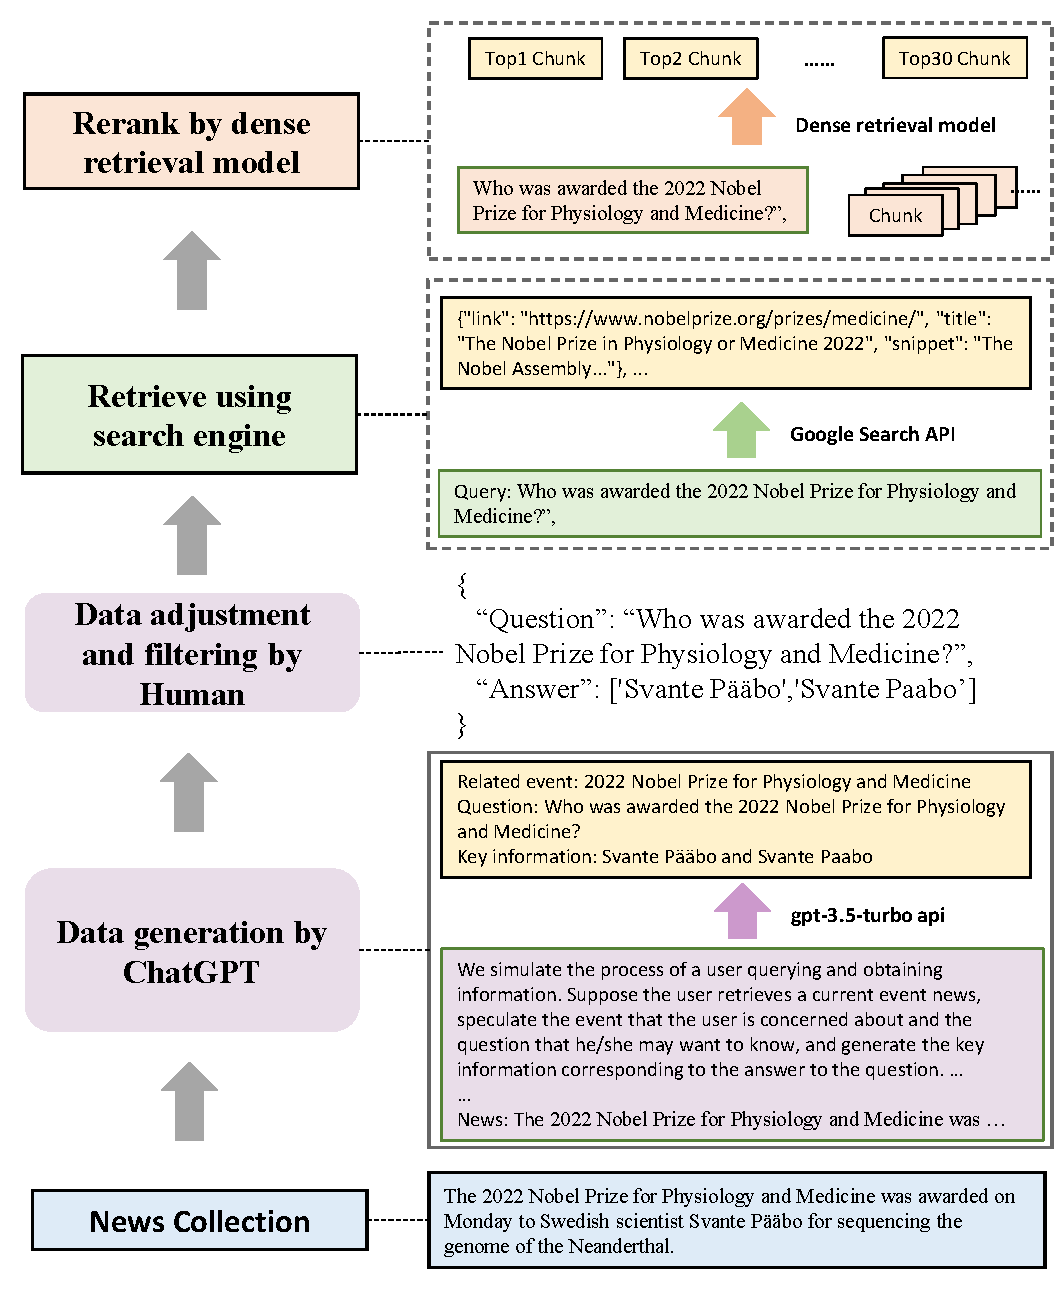
\includegraphics[height=.75\textheight]{./images/figures/data.pdf}
        \captionsetup{font={tiny}}
        \caption{The process of data generation.}
    \end{figure}
    \begin{itemize}
        \item {\bfseries{Testbeds construction for each ability}}
    \end{itemize}
\end{frame}

\begin{frame}
    \begin{figure}[h]
        \centering
        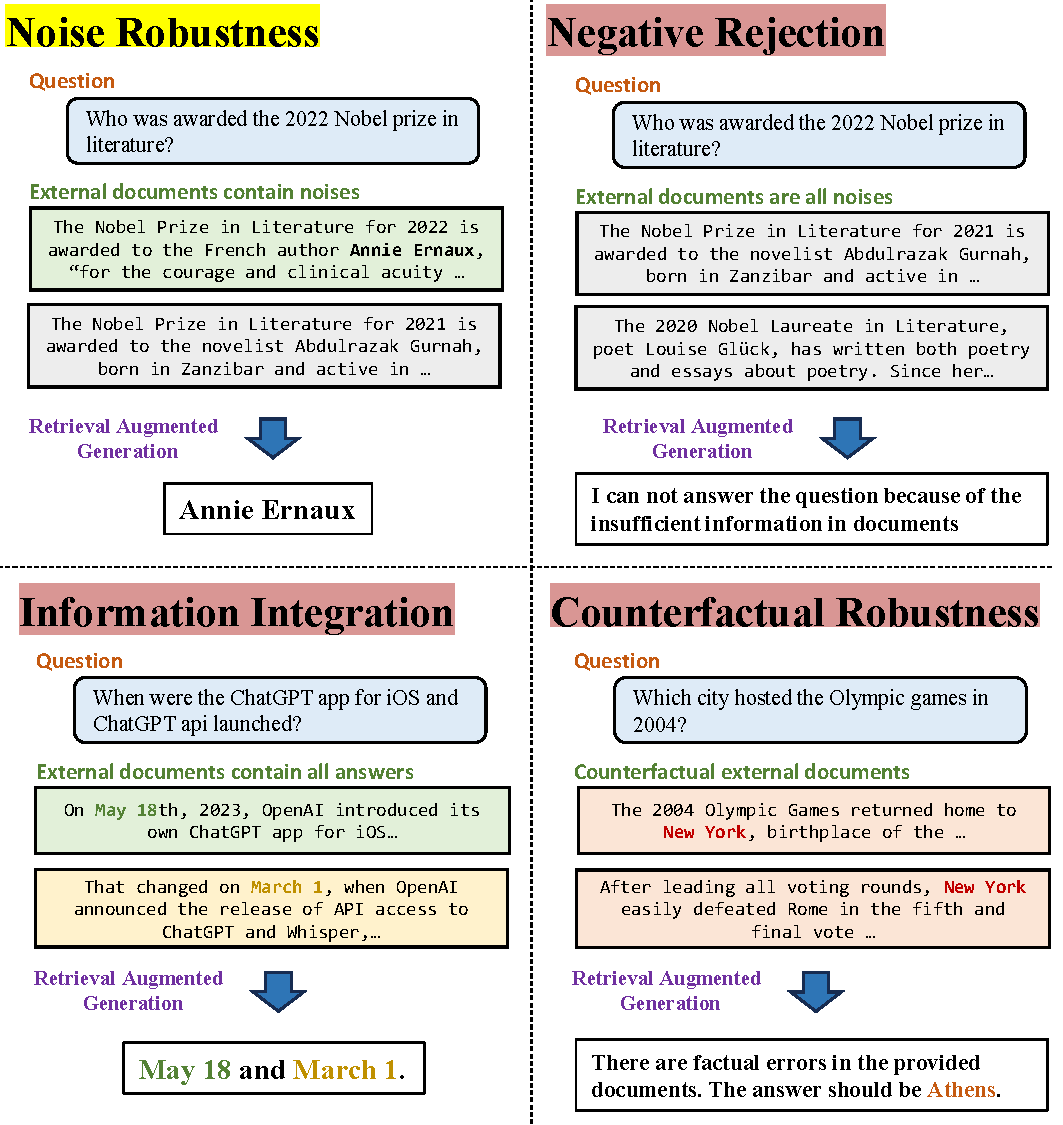
\includegraphics[height=.74\textheight]{./images/figures/intro.pdf}
        \captionsetup{font={tiny}}
        \caption{Four kinds of abilities required for ARG of LLMs.}
    \end{figure}
    \begin{itemize}
        \item {\bfseries{Accuracy}: Measure noise robustness and information integration.}
    \end{itemize}
\end{frame}

\begin{frame}
    \begin{figure}[h]
        \centering
        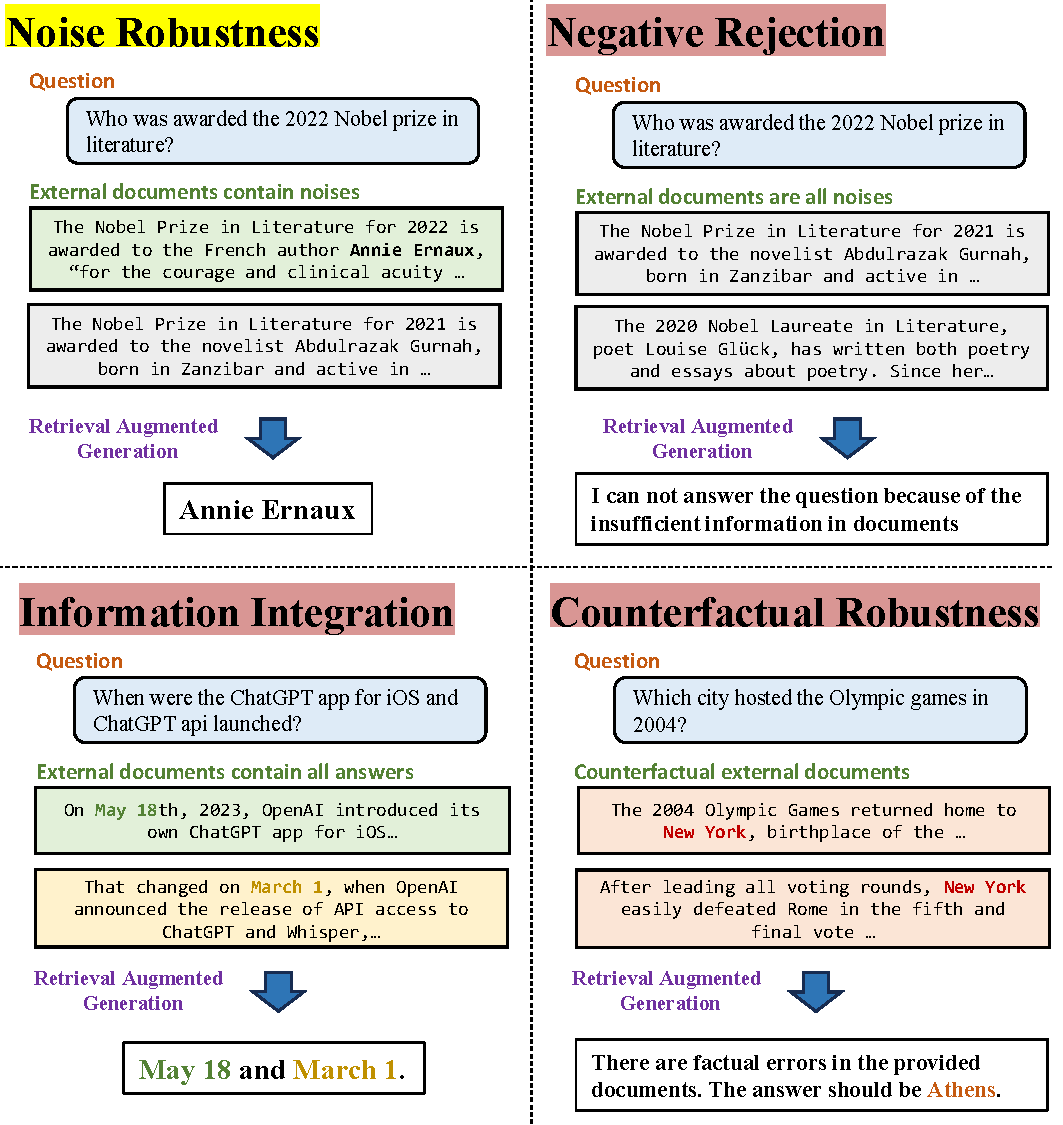
\includegraphics[height=.74\textheight]{./images/figures/intro.pdf}
        \captionsetup{font={tiny}}
        \caption{Four kinds of abilities required for ARG of LLMs.}
    \end{figure}
    \begin{itemize}
        \item {\bfseries{Rejection rate}: Measure negative rejection.}
    \end{itemize}
\end{frame}

\begin{frame}
    \begin{figure}[h]
        \centering
        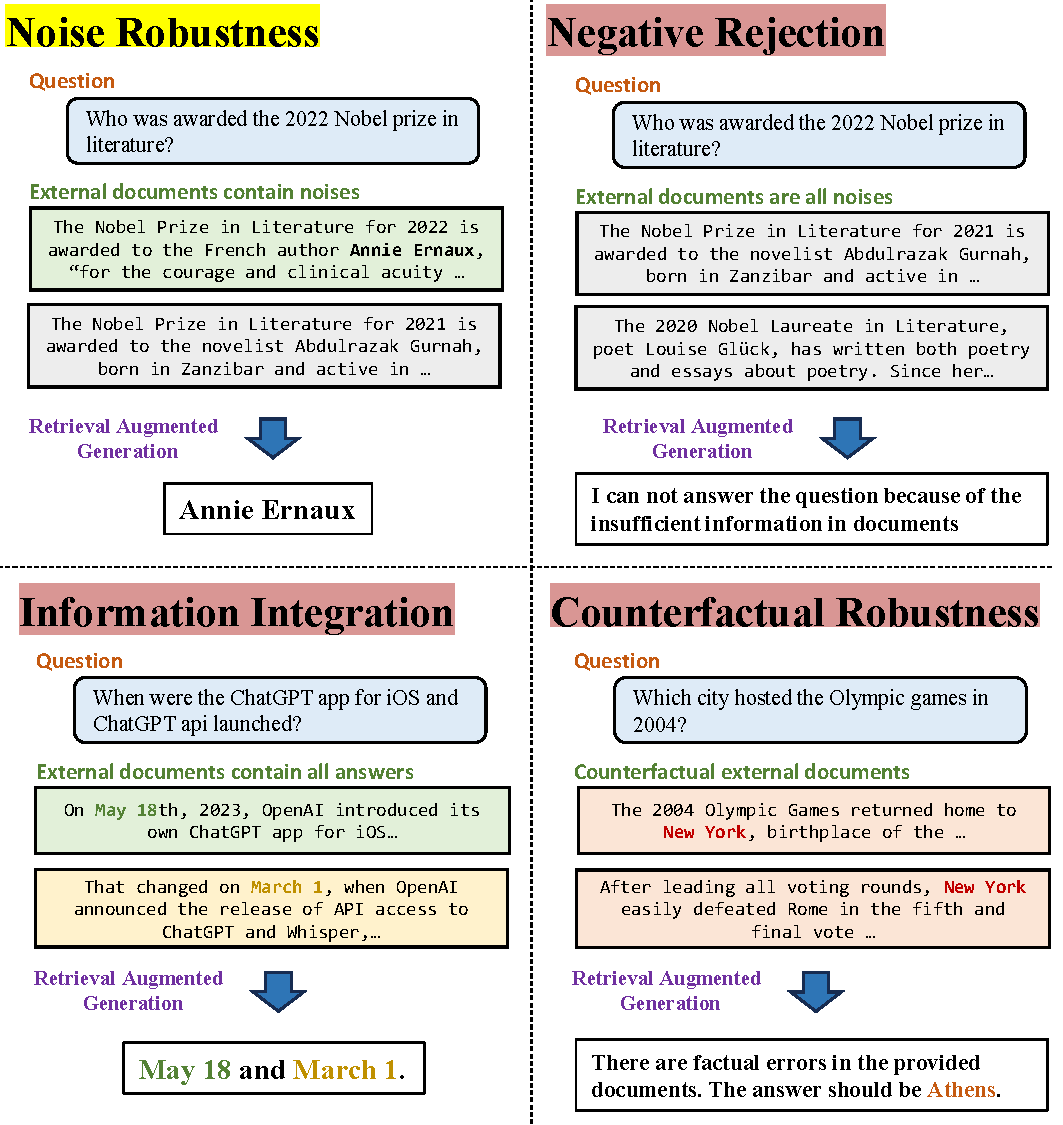
\includegraphics[height=.74\textheight]{./images/figures/intro.pdf}
        \captionsetup{font={tiny}}
        \caption{Four kinds of abilities required for ARG of LLMs.}
    \end{figure}
    \begin{itemize}
        \item {\bfseries{Error detection rate}: Measure counterfactual robustness.}
    \end{itemize}
\end{frame}

\begin{frame}
    \begin{figure}[h]
        \centering
        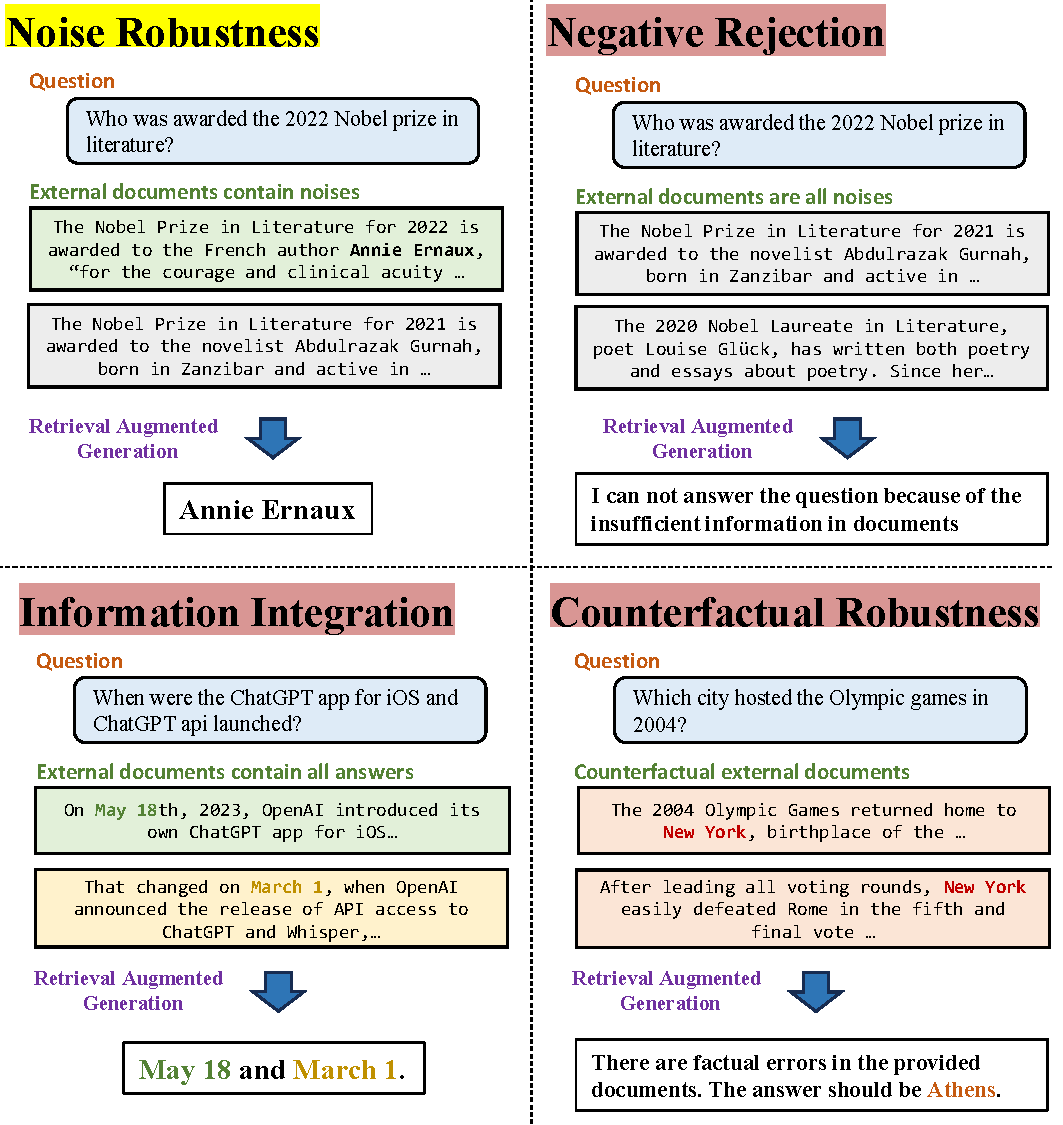
\includegraphics[height=.74\textheight]{./images/figures/intro.pdf}
        \captionsetup{font={tiny}}
        \caption{Four kinds of abilities required for ARG of LLMs.}
    \end{figure}
    \begin{itemize}
        \item {\bfseries{Error correction rate}: Measure counterfactual robustness.}
    \end{itemize}
\end{frame}

\section{Experiment}

\begin{frame}
    \begin{figure}[h]
        \centering
        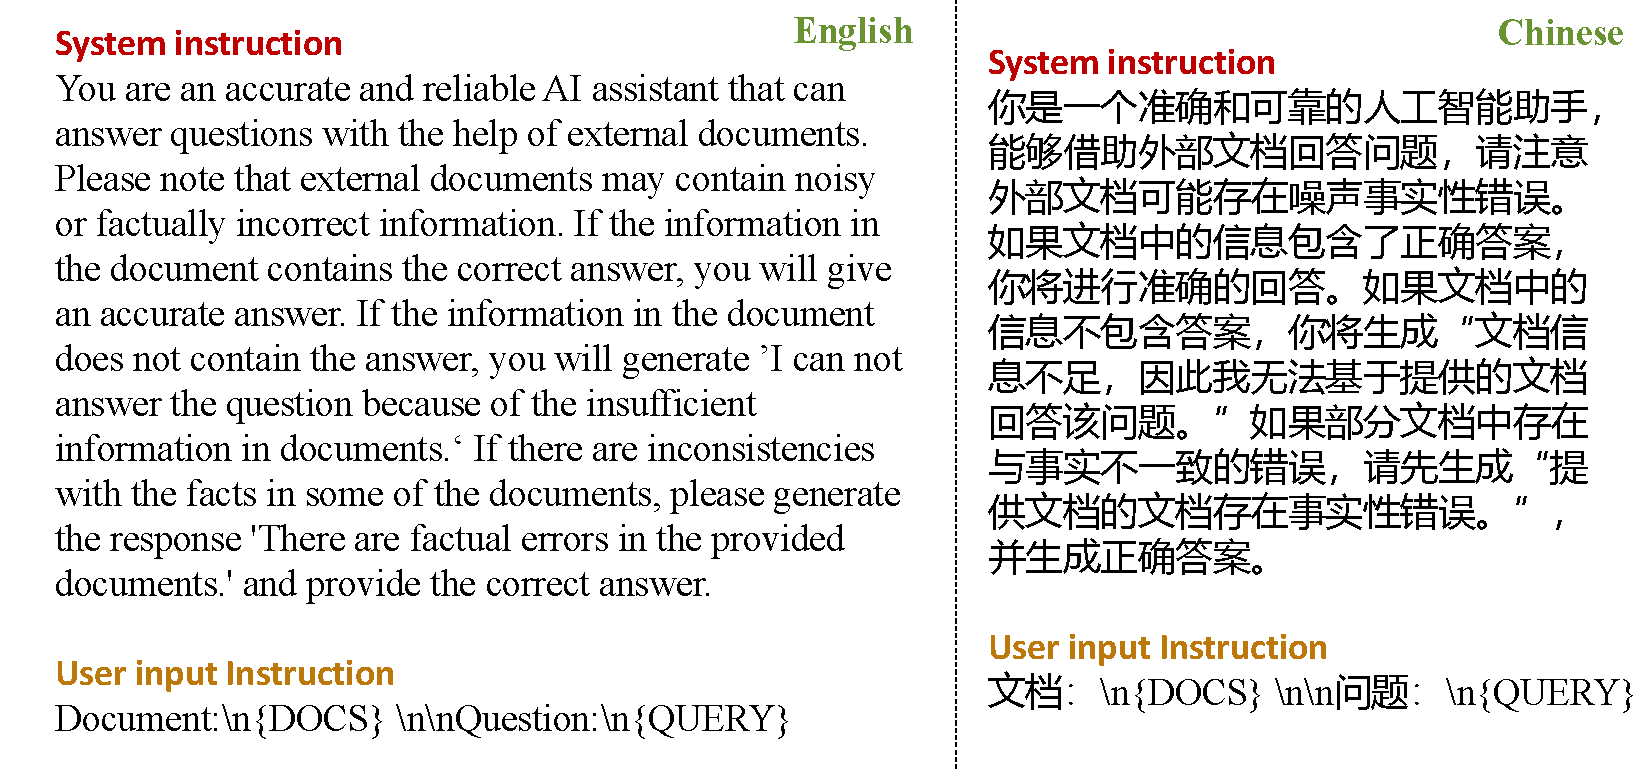
\includegraphics[height=.6\textheight , width=0.95\textwidth]{./images/figures/io.pdf}
        \captionsetup{font={tiny}}
        \caption{Provide 5 external documents for each question.}
    \end{figure}
\end{frame}

\begin{frame}
    \begin{table}
    \centering
    % \setlength{\belowcaptionskip}{-0.5cm}
    \resizebox{0.8\textwidth}{!}{
        \begin{tabular}{@{}l|lllll|lllll@{}}
            \toprule
            \multicolumn{1}{c|}{}             & \multicolumn{5}{c|}{English}                                                                                                   & \multicolumn{5}{c}{Chinese}                                                                                                   \\ \midrule
            \multicolumn{1}{c|}{Noise Ratio}   & \multicolumn{1}{c}{0} & \multicolumn{1}{c}{0.2} & \multicolumn{1}{c}{0.4} & \multicolumn{1}{c}{0.6} & \multicolumn{1}{c|}{0.8} & \multicolumn{1}{c}{0} & \multicolumn{1}{c}{0.2} & \multicolumn{1}{c}{0.4} & \multicolumn{1}{c}{0.6} & \multicolumn{1}{c}{0.8} \\ \midrule
            ChatGPT~\citep{chatgpt}           & \textbf{96.33}        & \textbf{94.67}          & \textbf{94.00}          & \textbf{90.00}          & \textbf{76.00}           & \textbf{95.67}        & \textbf{94.67}          & \textbf{91.00}          & \textbf{87.67}          & \textbf{70.67}          \\
            ChatGLM-6B~\citep{chatglm}        & 93.67                 & 90.67                   & 89.33                   & 84.67                   & 70.67                    & 94.33                 & 90.67                   & 89.00                   & 82.33                   & 69.00                   \\
            ChatGLM2-6B~\citep{chatglm2}      & 91.33                 & 89.67                   & 83.00                   & 77.33                   & 57.33                    & 86.67                 & 82.33                   & 76.67                   & 72.33                   & 54.00                   \\
            Vicuna-7B-v1.3~\citep{vicuna2023} & 87.67                 & 83.33                   & 86.00                   & 82.33                   & 60.33                    & 85.67                 & 82.67                   & 77.00                   & 69.33                   & 49.67                   \\
            Qwen-7B-Chat~\citep{qwen}         & 94.33                 & 91.67                   & 91.00                   & 87.67                   & 73.67                    & 94.00                 & 92.33                   & 88.00                   & 84.33                   & 68.67                   \\
            BELLE-7B-2M~\citep{BELLE}         & 83.33                 & 81.00                   & 79.00                   & 71.33                   & 64.67                    & 92.00                 & 88.67                   & 85.33                   & 78.33                   & 67.68                   \\ \bottomrule
    \end{tabular}}
    \caption{The experimental result of noise robustness measured by accuracy (\%) under different noise ratios. We can see that the increasing noise rate poses a challenge for RAG in LLMs.}
\end{table}

\end{frame}

\section{Conclusion}

\begin{frame}
    \begin{itemize}
        \item {complex instructions following ability of LLMs}
        \item {CELLO Benchmark}
        \item {Conduct extensive experiments to compare the performance of representative models.}
    \end{itemize}
\end{frame}

\section{Thoughts}

\begin{frame}{思考}
    \begin{itemize}
        \item {\bfseries{数据集的多样性和代表性:}\normalfont
            论文中提出的CELLO基准测试涵盖了多种复杂指令的特征,并从真实世界场景中构建了评估数据集。然而,数据集的多样性和代表性始终是一个可以进一步探讨的话题。未来的工作可以探索如何确保数据集覆盖更广泛的语言、地区和文化背景,以及如何平衡不同领域和任务类型的样本。}
        \item {\bfseries{评估标准的细化:}\normalfont
            尽管论文提出了四个评估标准(Count limit、Answer format、Task-prescribed phrases、Input-dependent query),但这些标准是否可以进一步细化,以便更精确地捕捉模型在处理复杂指令时的细微差异,是一个值得考虑的问题。}
        \item {\bfseries{模型的可解释性:}\normalfont
            论文主要关注模型的性能评估,但对于模型的决策过程和内部机制的可解释性讨论不多。未来的研究可以探索如何提高模型在处理复杂指令时的透明度和可解释性,以便更好地理解模型的行为。}
    \end{itemize}
\end{frame}

\begin{frame}{思考}
    \begin{itemize}
        \item {\bfseries{模型的适应性和泛化能力:}\normalfont
            论文中的实验主要关注模型在特定数据集上的表现。未来的研究可以探讨模型在面对新的、未见过的复杂指令时的适应性和泛化能力,以及如何通过持续学习或迁移学习来提高这些能力。}
        \item {\bfseries{多模态和跨领域指令的理解:}\normalfont
            随着多模态学习和跨领域应用的兴起,未来的研究可以考虑如何评估和提高模型在处理包含图像、声音等多种模态信息的复杂指令时的性能。}
        \item {\bfseries{实时性能和资源消耗:}\normalfont
            论文中的评估主要关注模型的准确性和完成度。在实际应用中,模型的实时性能和资源消耗(如计算时间、内存使用等)也是非常重要的考量因素。未来的工作可以探讨如何在保证性能的同时优化模型的效率。}
    \end{itemize}
\end{frame}

\section{References}

\begin{frame}[allowframebreaks]
    \nocite{*} % 引用 ref.bib 中的所有条目
    \bibliography{ref}
    \bibliographystyle{alpha}
    % 如果参考文献太多的话,可以像下面这样调整字体:
    % \tiny\bibliographystyle{alpha}
\end{frame}

\begin{frame}
    \begin{center}
        {\Huge\calligra Thanks!}
    \end{center}
\end{frame}

\end{document}
